\sectionframe{Background of my Masters Thesis}
\section{Background}

\begin{frame}{Continuous Model}
    \vspace{-1em}
    \begin{columns}
        \begin{column}{.4 \textwidth}
            \begin{itemize}
                \item DC/AC power converter
                \item Variable switching
            \end{itemize}
        \end{column}
        \begin{column}{.6 \textwidth}
            \begin{figure}
                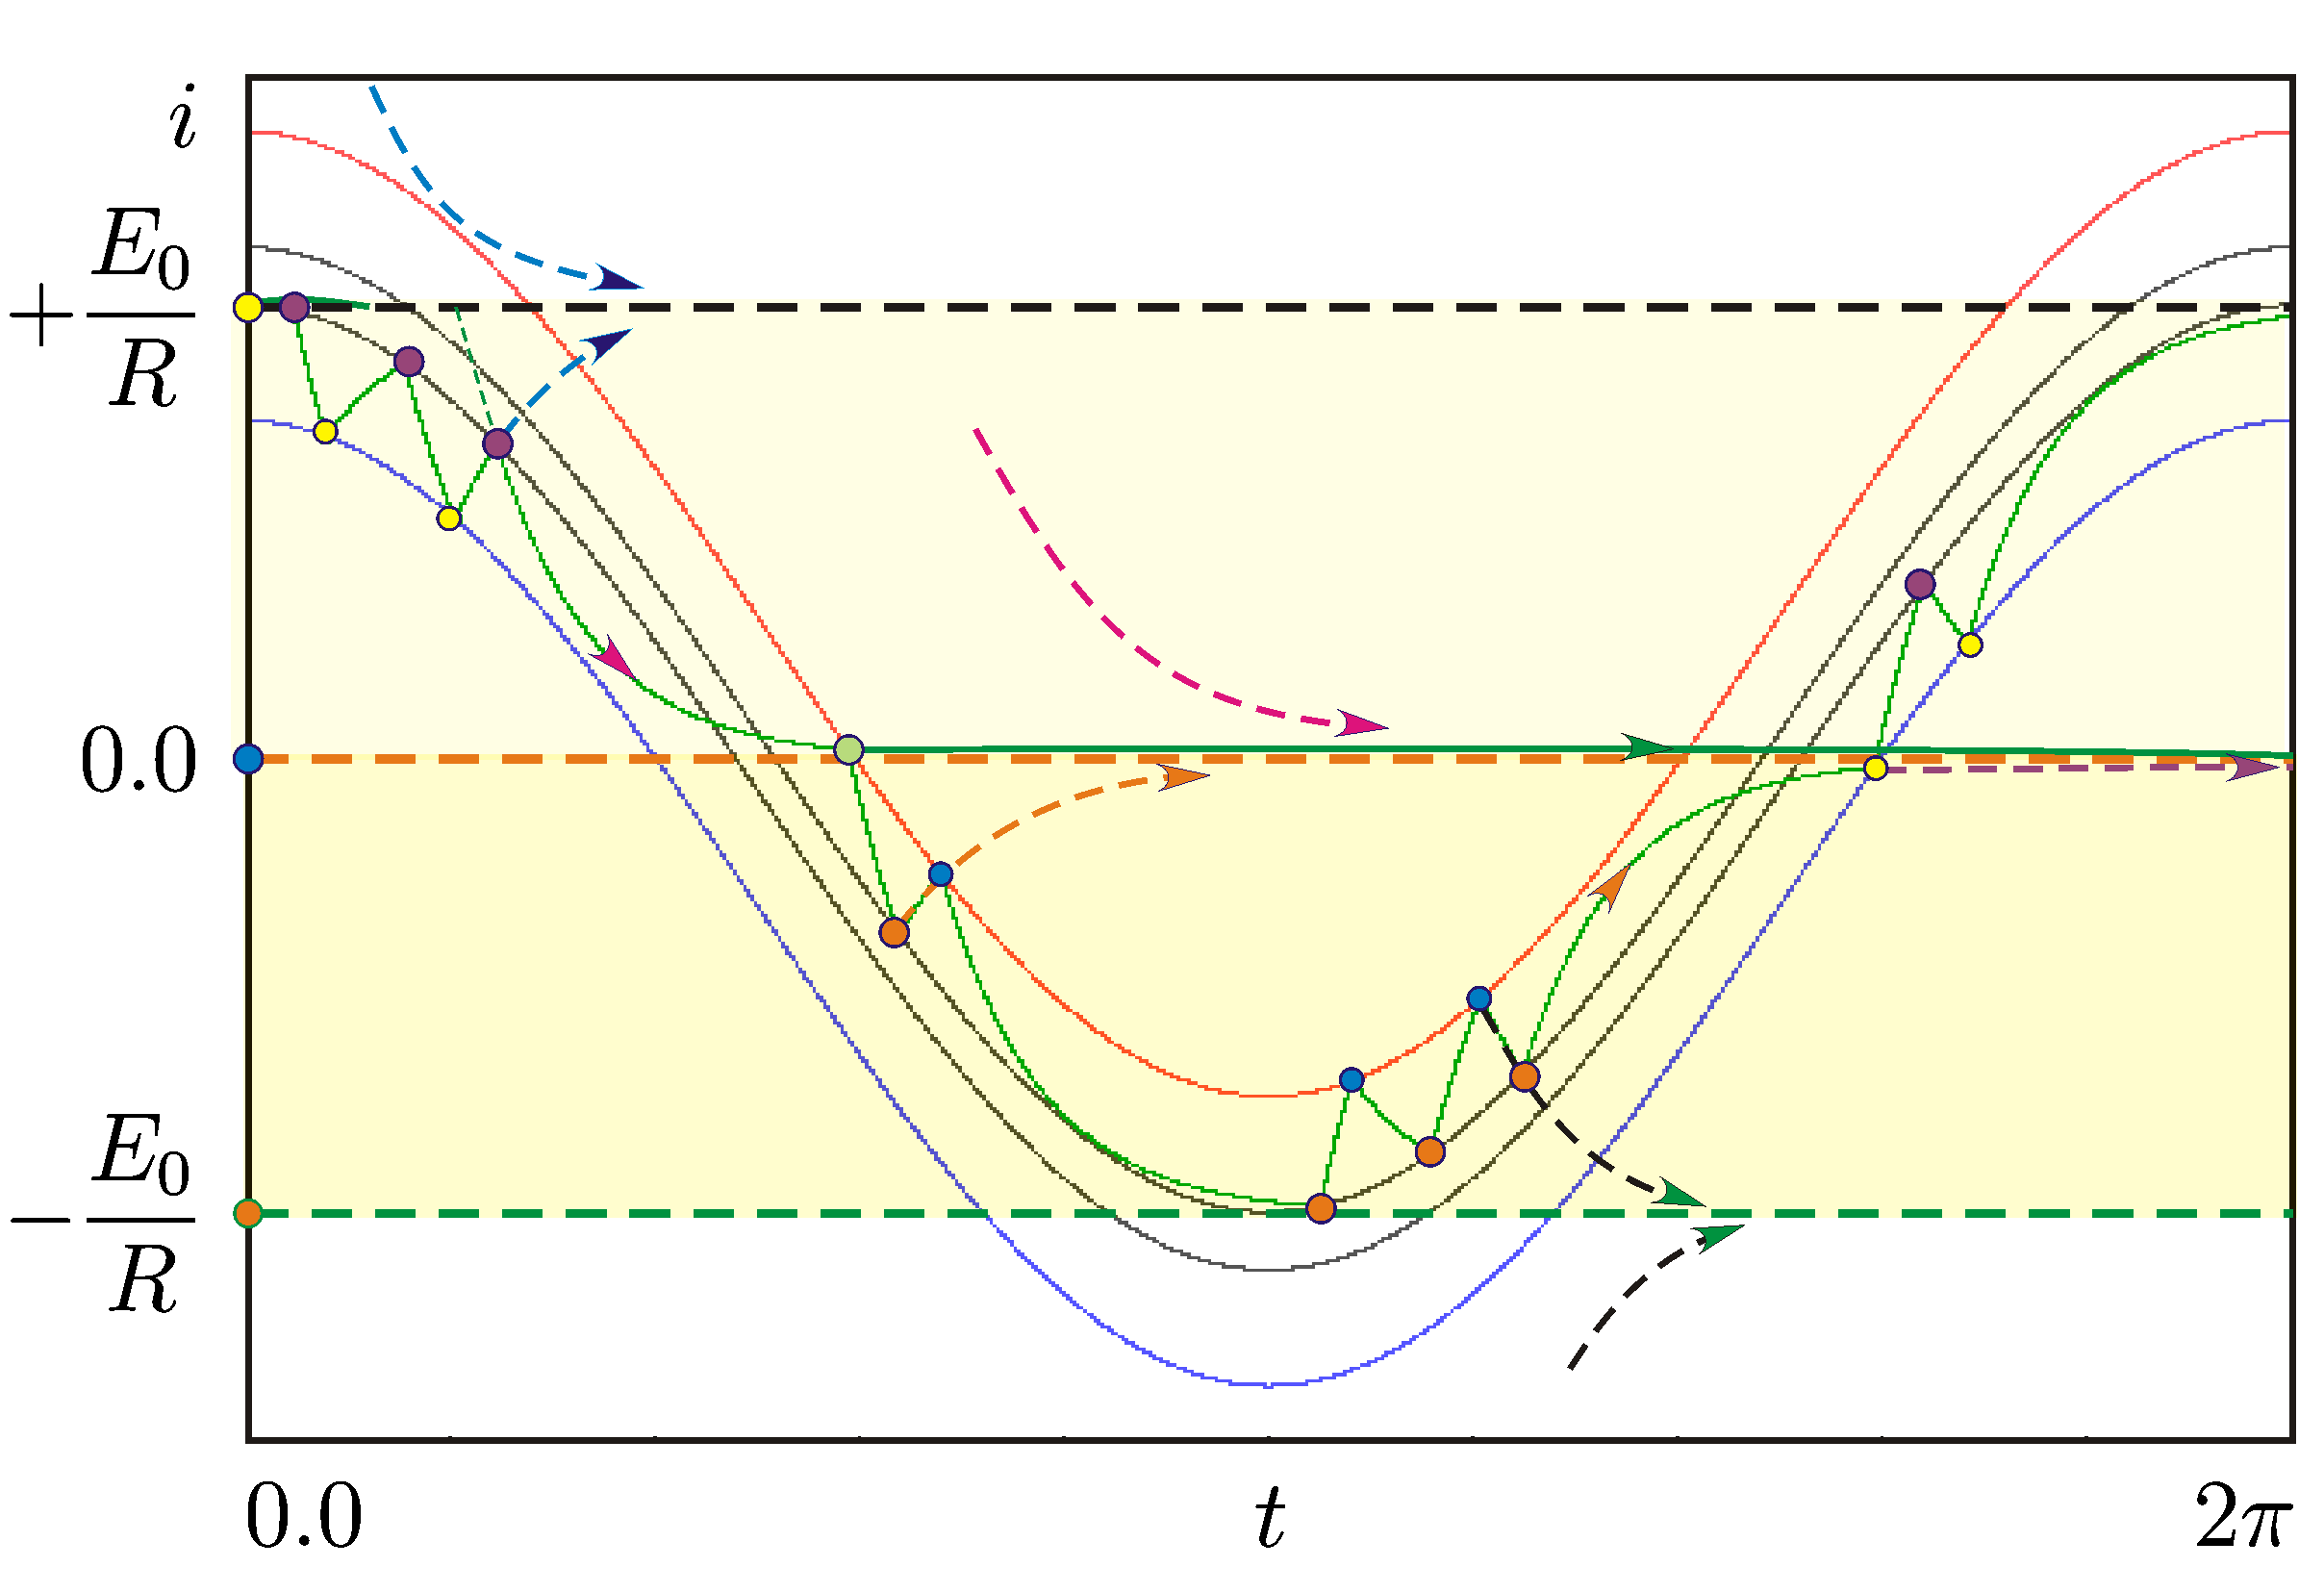
\includegraphics[width=0.8 \textwidth]{Figs/continuous_model.png}
            \end{figure}

            \flushright{[Zhusubaliyev]}
        \end{column}
    \end{columns}
\end{frame}

\begin{frame}{Discrete Model}
    \vspace{-2em}
    \begin{align*}
        \tau_{n+1} & =  F(\tau_n) \mod 2 \pi
        \\
        F(\tau)    & = \begin{cases}
                            F_1(\tau) & \text{if } q \cdot \cos(\tau) > 0 \\
                            F_2(\tau) & \text{if } q \cdot \cos(\tau) < 0
                        \end{cases}
        \\
        F_1(\tau)  & = \begin{cases}
                            \tau + z^{+} + z_{1}^{+}     & \text{if } z^{+} < z_{0}^{+} \\
                            \tau + z_{0}^{+} + z_{2}^{+} & \text{if } z^{+} > z_{0}^{+}
                        \end{cases}
        \\
        F_2(\tau)  & = \begin{cases}
                            \tau + z^{-} + z_{1}^{-}     & \text{if } z^{-} < z_{0}^{-} \\
                            \tau + z_{0}^{-} + z_{2}^{-} & \text{if } z^{-} > z_{0}^{-}
                        \end{cases}
    \end{align*}

    \vspace{1em}
    Values of $ z^{+}, z_{1}^{+}, z_{0}^{+}, z_{2}^{+}, z^{-}, z_{1}^{-}, z_{0}^{-}, \text{ and } z_{2}^{-}$?
\end{frame}

\begin{frame}{Discrete Model}
    \vspace{-3em}
    \begin{align*}
        (q \cdot \cos(\tau) - \chi_{c}) \cdot e^{\lambda \cdot z^{+}}
            & = q \cdot \cos(\tau + z^{+}) - \chi_{0}                  \\
        (q \cdot \cos(\tau + z^{+}) - \chi_{0} - 1) \cdot e^{\lambda \cdot z_{1}^{+}} + 1
            & = q \cdot  \cos(\tau + z^{+} + z_{1}^{+}) - \chi_{c}     \\
        (q \cdot \cos(\tau) - \chi_{c}) \cdot e^{\lambda \cdot z_{0}^{+}}
            & = q \cdot \cos(\tau + z_{0}^{+}) + \chi_{0}              \\
        (q \cdot \cos(\tau + z_{0}^{+} + z_{2}^{+}) + \chi_{0} + 1) \cdot e^{\lambda \cdot z_{2}^{+}} - 1
            & = q \cdot  \cos(\tau + z_{0}^{+} + z_{2}^{+}) + \chi_{c} \\[1em]
        (q \cdot \cos(\tau) + \chi_{c}) \cdot e^{\lambda \cdot z^{-}}
            & = q \cdot \cos(\tau + z^{-}) + \chi_{0}                  \\
        (q \cdot \cos(\tau + z^{-}) + \chi_{0} + 1) \cdot e^{\lambda \cdot z_{1}^{-}} - 1
            & = q \cdot  \cos(\tau + z^{-} + z_{1}^{-}) + \chi_{c}     \\
        (q \cdot \cos(\tau) + \chi_{c}) \cdot e^{\lambda \cdot z_{0}^{-}}
            & = q \cdot \cos(\tau + z_{0}^{-}) - \chi_{0}              \\
        (q \cdot \cos(\tau + z_{0}^{-} + z_{2}^{-}) - \chi_{0} - 1) \cdot e^{\lambda \cdot z_{2}^{-}} + 1
            & = q \cdot  \cos(\tau + z_{0}^{-} + z_{2}^{-}) - \chi_{c} \\
    \end{align*}
    \vspace{-3em}
    \begin{flushright}
        Smallest positive solutions
        \hfill
        [Akyuz, Avrutin]
    \end{flushright}
\end{frame}

\begin{frame}{Unusual Bifurcation Structure}
    \begin{figure}
        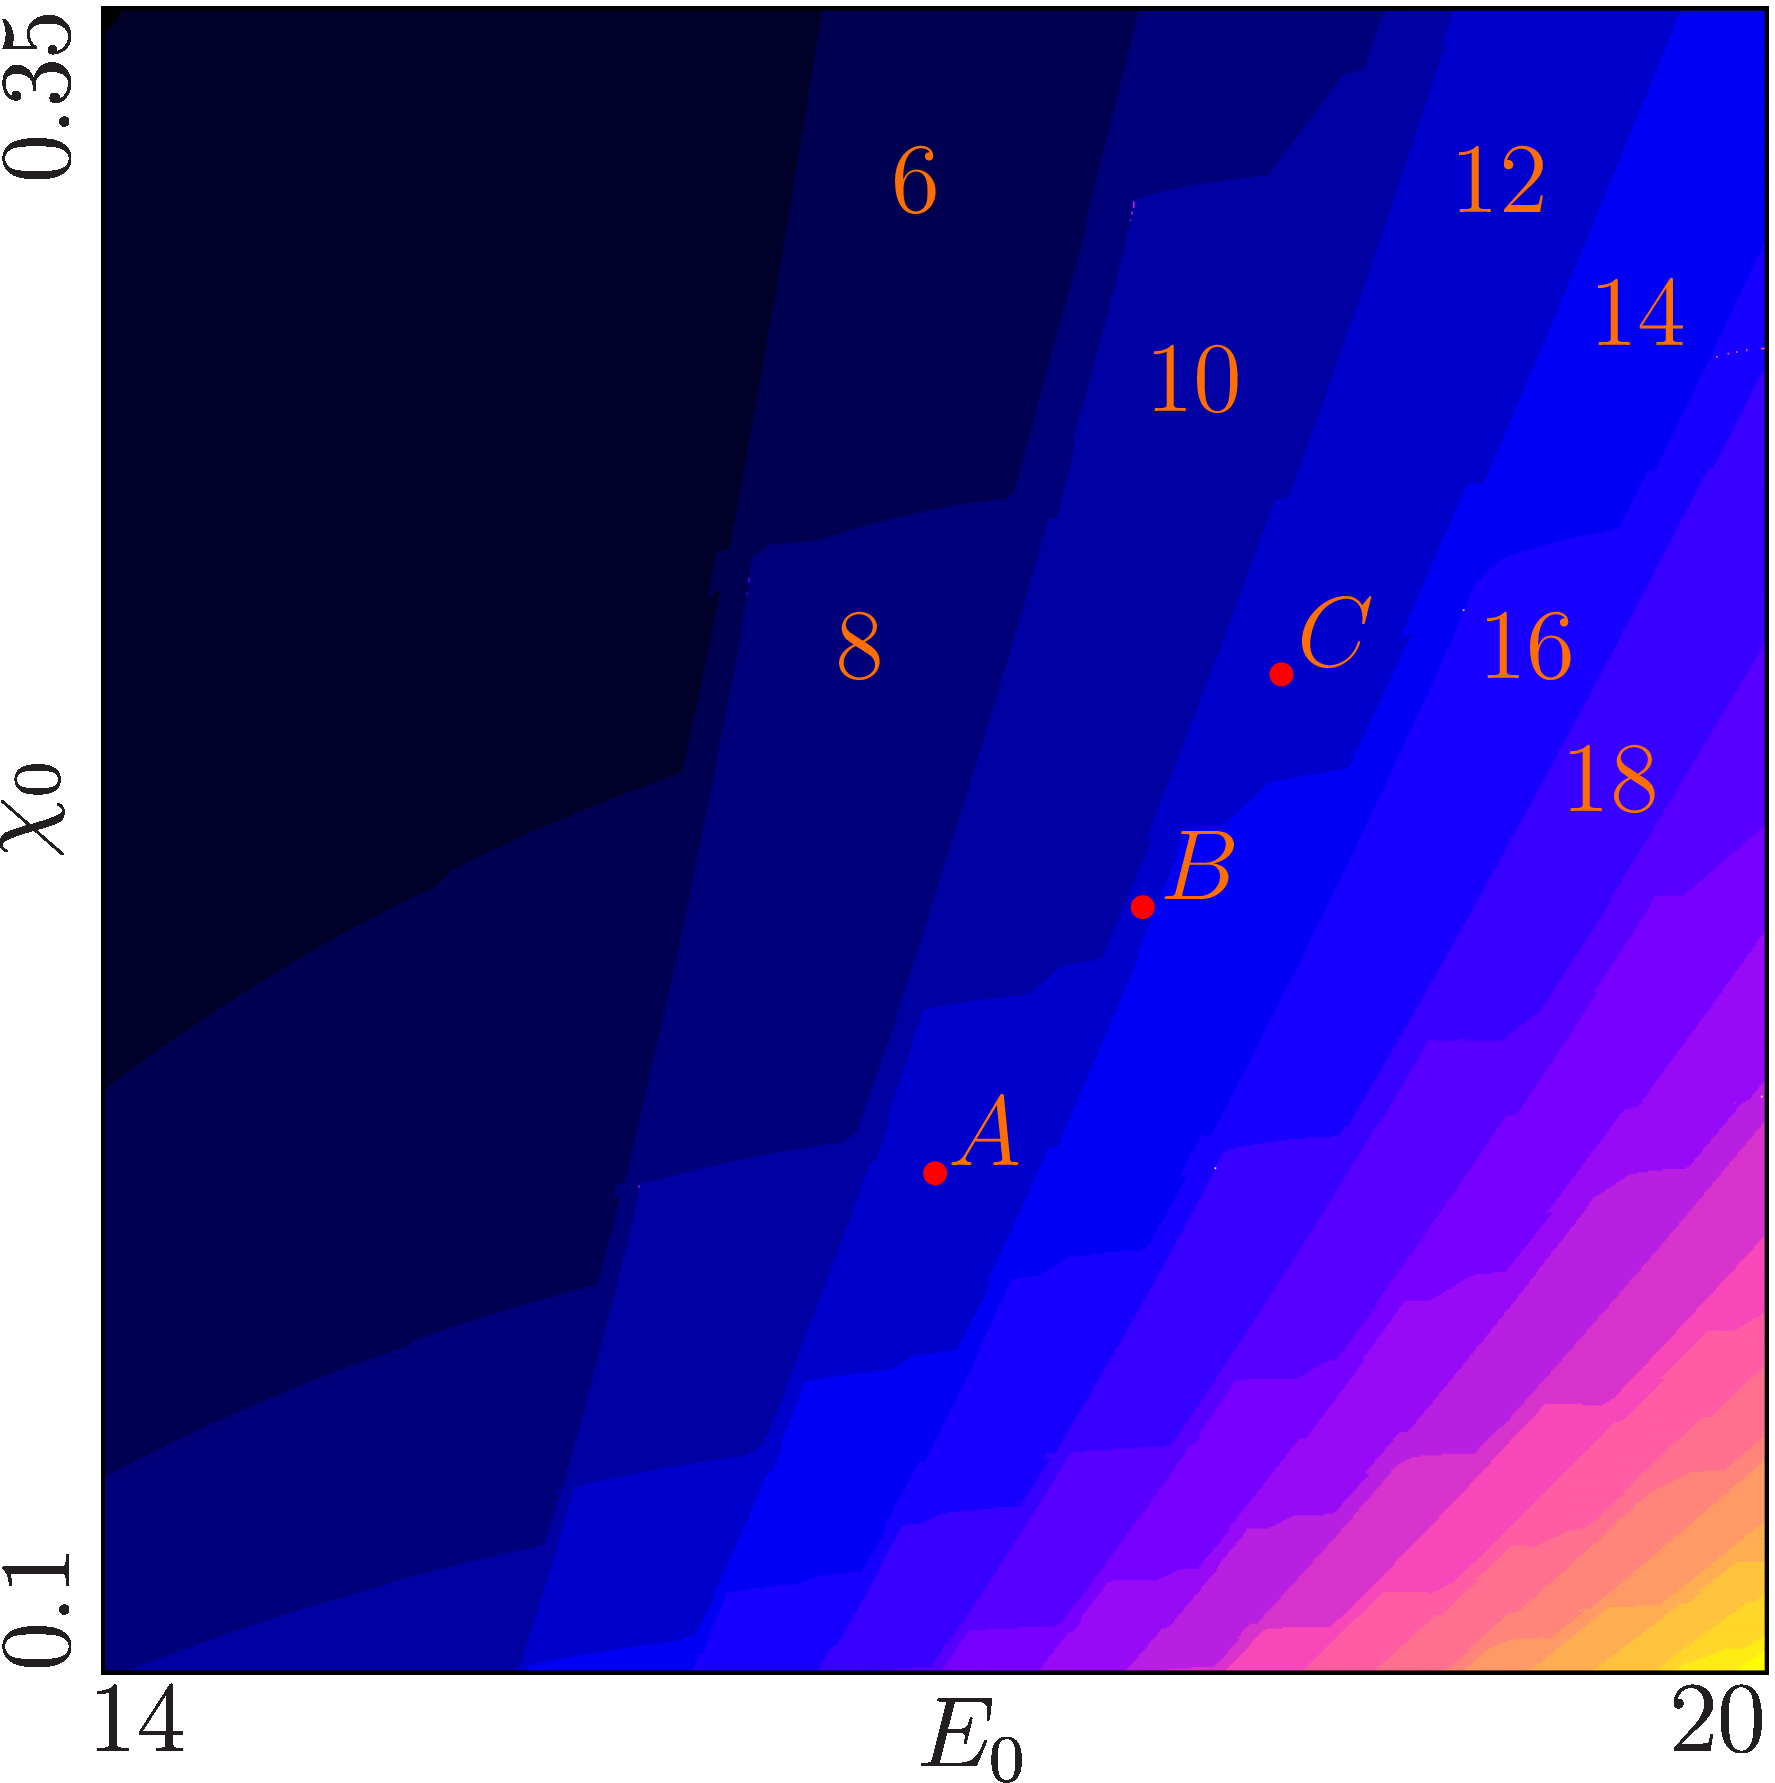
\includegraphics[width=0.45 \textwidth]{Figs/og_model_period.png}
    \end{figure}
\end{frame}

\begin{frame}{Unusual Bifurcation Structure}
    \begin{figure}
        \stackunder[5pt]{
            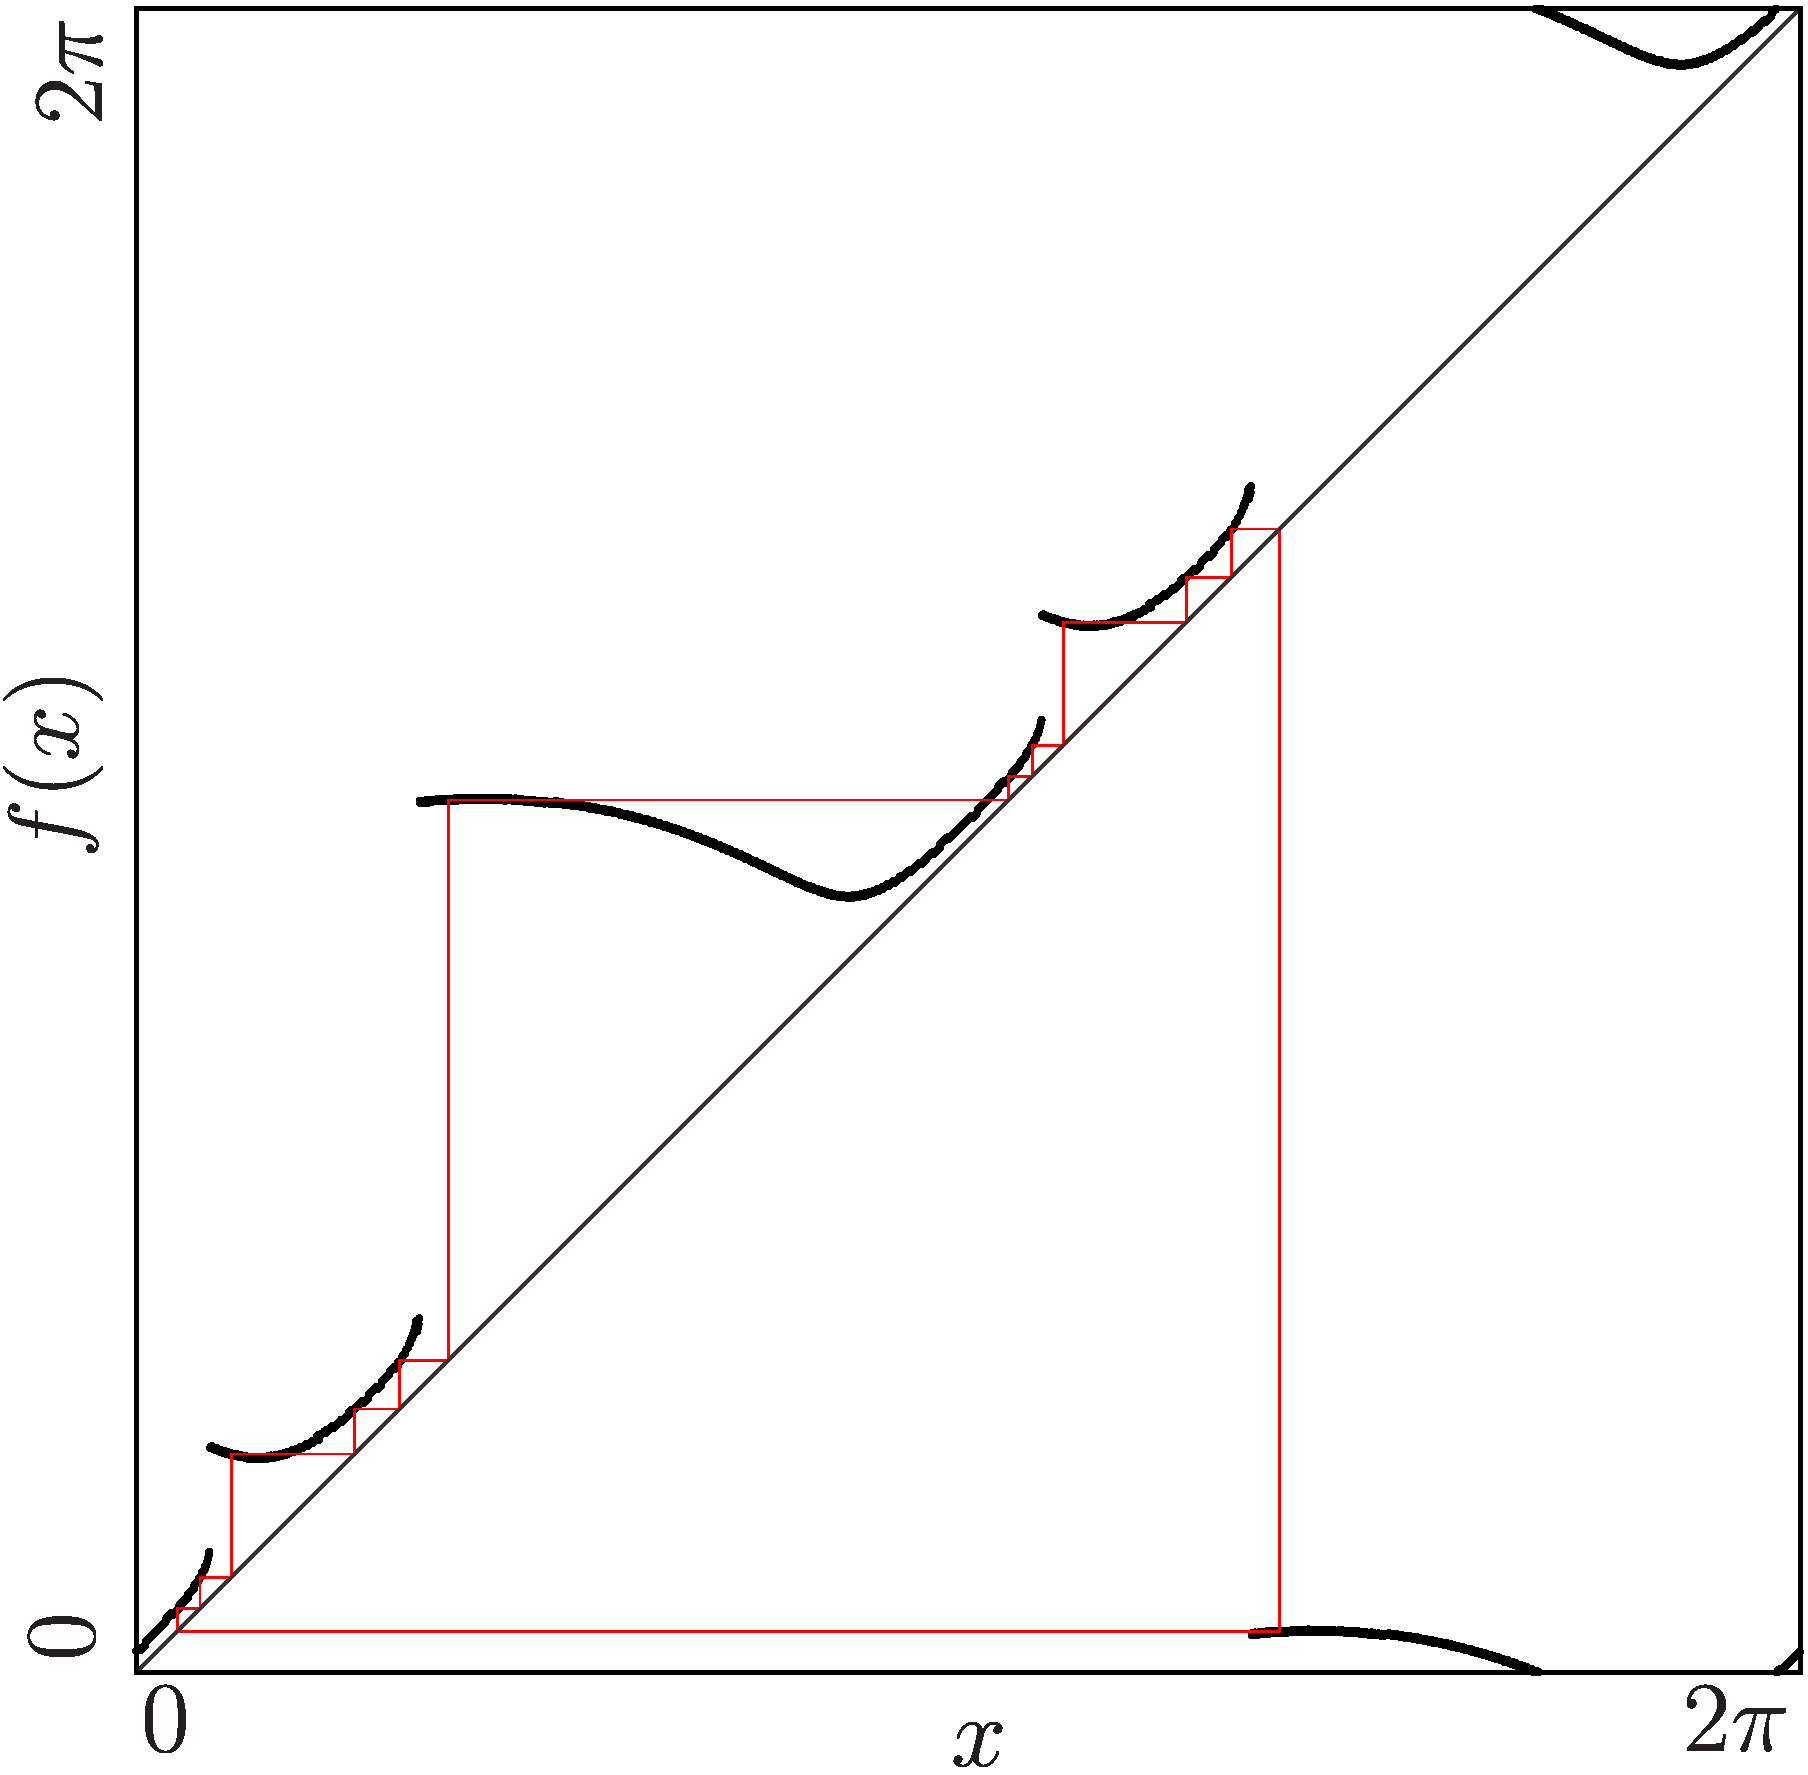
\includegraphics[width=0.3 \textwidth]{Figs/og_model_cycle_a.png}
        }{$\A^3\B^3\C^3\D^3$}
        \stackunder[5pt]{
            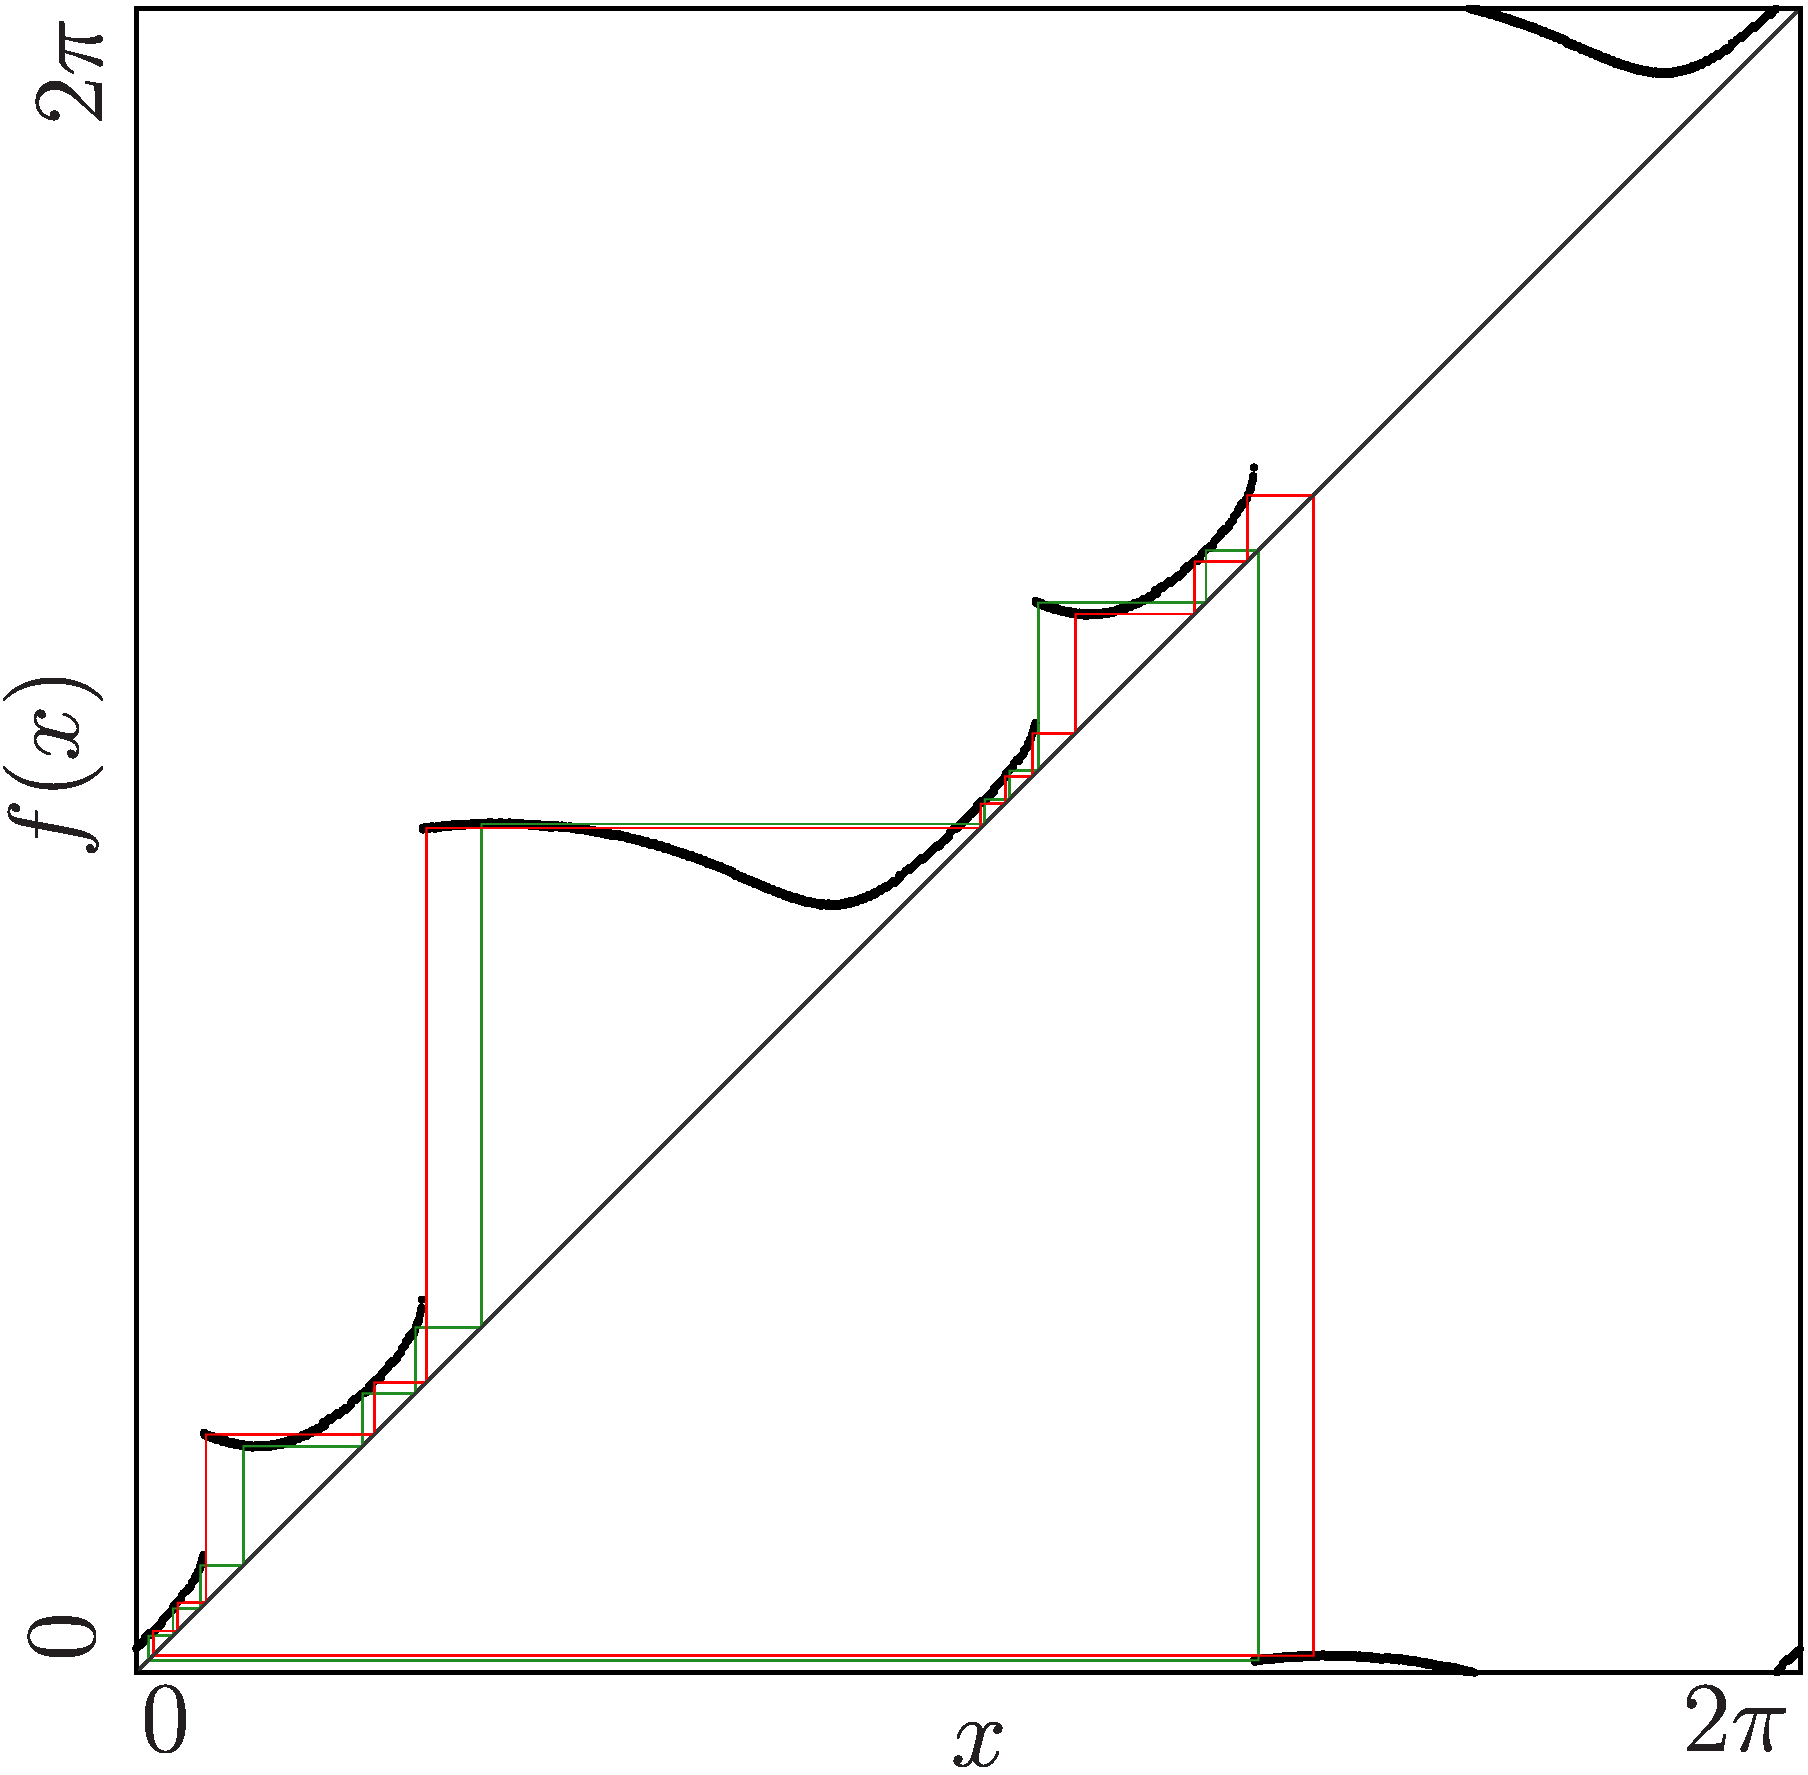
\includegraphics[width=0.3 \textwidth]{Figs/og_model_cycle_b.png}
        }{$\A^3\B^3\C^2\D^4,\:\A^2\B^4\C^3\D^3$}
        \stackunder[5pt]{
            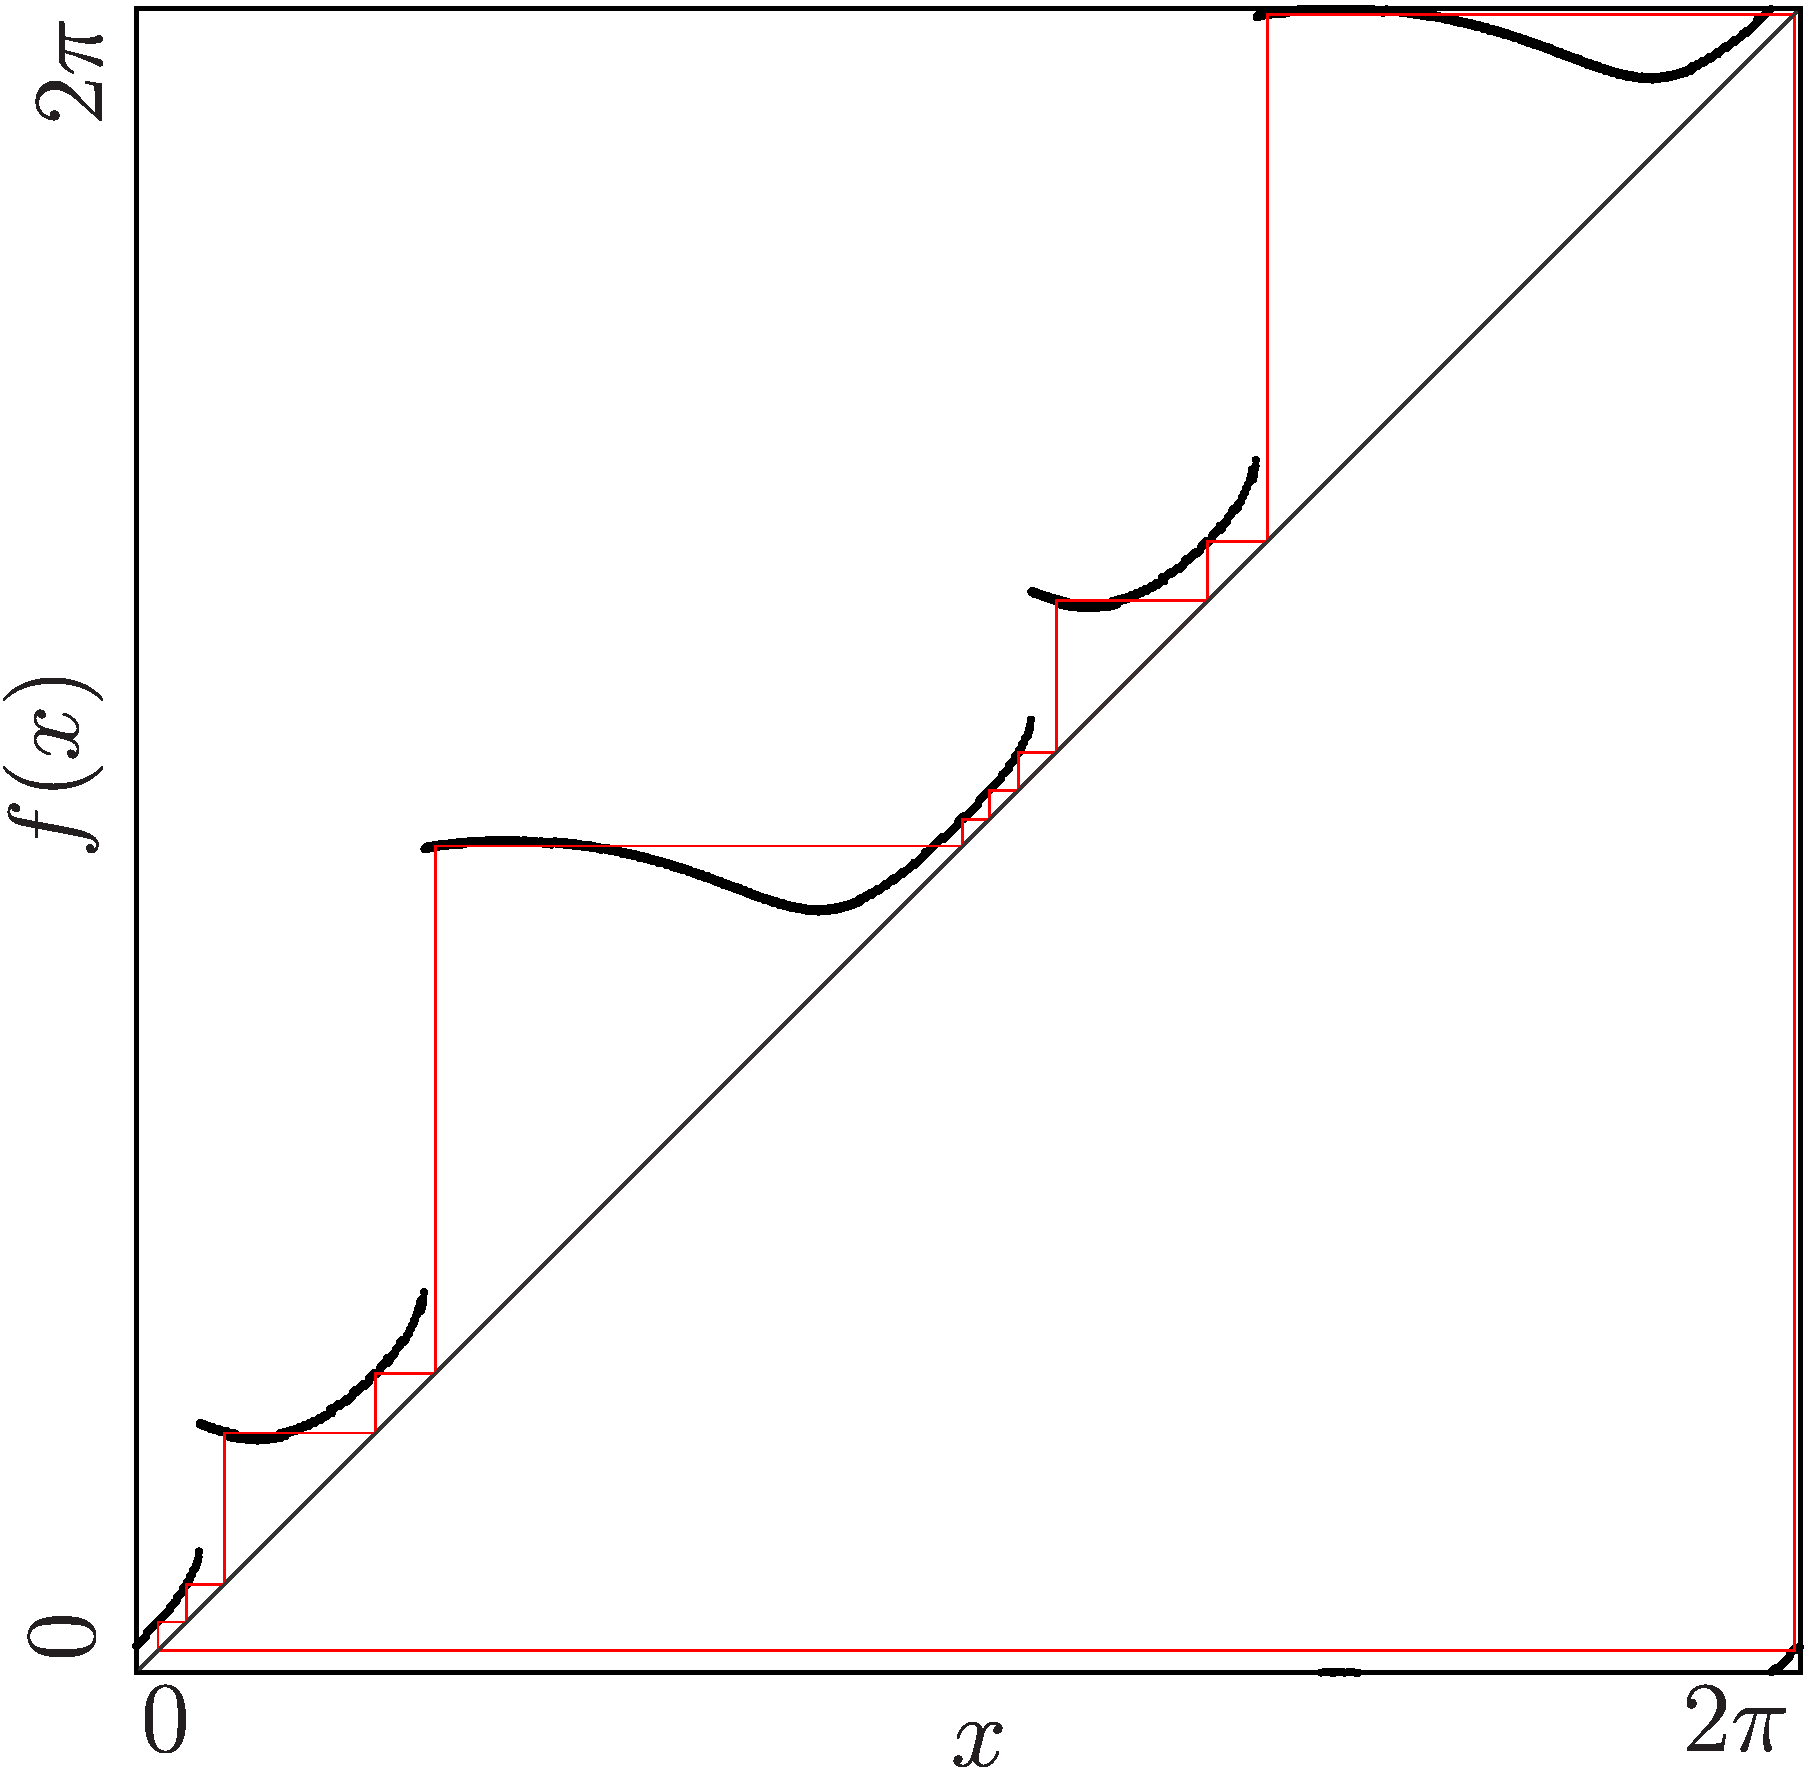
\includegraphics[width=0.3 \textwidth]{Figs/og_model_cycle_c.png}
        }{$\A^2\B^4\C^2\D^4$}
    \end{figure}

    \vspace{1em}
    Symmetry $F(\theta + \pi) = F(\theta) + \pi \mod 2\pi$ \hfill [Akyuz] %\cite{akyuz2022}
\end{frame}

%%% Local Variables:
%%% mode: latex
%%% TeX-master: "../Vortrag_Frauenhofer_Weik"
%%% End:
